% Chapter Template

\chapter{Lorenz System of Differential Equations and the Lorenz Attractor} % Main chapter title

\label{ChapterX} % Change X to a consecutive number; for referencing this chapter elsewhere, use \ref{ChapterX}

\lhead{Chapter 3. \emph{Lorenz System of Differential Equations and the Lorenz Attractor}} % Change X to a consecutive number; this is for the header on each page - perhaps a shortened title

The Lorenz system\cite{lorenz_1963} is described as follows :-
$$\dot{x} = \sigma(y-x)$$
$$\dot{y} = rx - y - xz$$
$$\dot{z} = xy - bz$$,
where $x,y,z$ are dynamical variables and $\sigma,r,b$ are constants.

These innocuous looking equations hold many secrets in them. The landmark 1963 paper by Lorenz describing these equations was written keeping in mind a convective model of atmospheric dynamics, but it has since found a wide variety of applications in lasers, circuits etc.

\section{A Few Properties}
\begin{itemize}
	\item Though the equations look simple, we can already see that the solutions might be complicated due to the nonlinearity in the terms $xy$ and $xz$. Nonlinear systems could lead to chaotic dynamics.
	\item One could try to solve these equations without much thought by putting it directly into a computer and getting a solution. But it is useful to note that the equation has a few symmetries. For example $(x,y,z) \rightarrow (-x,-y,z)$ keeps the solution invariant. This means that all solutions should be symmetric or have a redundant symmetric partner.
	\item One calls a system of equations dissipative if the phase space volume contracts as the system evolves in time. If we write the equations in a condensed form as $\dot{\boldsymbol{x}} = \boldsymbol{f}(\boldsymbol{x})$, then the volume the rate of change of volume is given by $\nabla.\boldsymbol{f}$ integrated over the volume. We can see
	$$\nabla.\boldsymbol{f} = \frac{\partial}{\partial x}[\sigma(y-x)] + \frac{\partial}{\partial y}[rx-y-xz] + \frac{\partial}{\partial z}[xy-bz] = -(\sigma +1 +b) < 0$$
	This is a negative constant. So, the phase space volume decreases in time and the Lorenz system is dissipative.
	\item Lets consider the Lorenz system without the nonlinearities. If one looks closely, this system is equivalent to linearizing the original system by considering perturbations around the origin. The equations would then read,
	\begin{eqnarray}
		\dot{x} = \sigma(y-x) \\
		\dot{y} = rx - y \\
		\dot{z} = - bz,
	\end{eqnarray}
	We can immediately see that the equation for $z$ is decoupled from the other two. Also, the $z$ solution decays exponentially as $t\rightarrow \infty$. The other two equations can be written as :-
	$$\left(\begin{array}{cc} \dot{x} \\\dot{y} \end{array}\right) = \left(\begin{array}{cc} -\sigma & \sigma \\\ r & -1 \end{array}\right) \left(\begin{array}{cc} x \\y \end{array}\right)$$
	The determinant $\Delta=-\sigma(1-r)$ and trace $\tau = -(\sigma+1)$. The system has a saddle point at $r>1$
\end{itemize}	
\section{Numerical Solution}
We have seen that a signature of chaos is that the trajectories diverge for a slight change in the initial conditions. As these equations are not really very straightforward to solve analytically, we solve it numerically using Python. We use initial conditions as $(1,1,1)$ and $(1.0000001,1,1)$, and plot the variation of $x,y,z$ with time $t$. 

Fig. [\ref{fig:dyvar_vs_t}] plots the numerically integrated equation for these slightly different initial conditions. We see that this system shows clear signs of chaos - the trajectories start diverging after $t=30$ or so. This is clearly evident from Fig. [\ref{fig:delta_trajectory}], which plots the deviation of paths from each other with time.

\begin{figure}[h!]
	\centering
	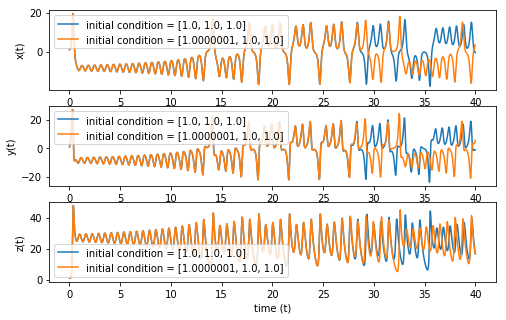
\includegraphics[scale=0.8]{Figures/dyvar_vs_t.png}
	\caption[An Electron]{Numerical solutions for different initial conditions. Trajectories start to visibly diverge roughly around $t=30$.}
	\label{fig:dyvar_vs_t}
\end{figure}

Typically, if we take the two initial conditions far away from each other, we will se that the system goes to chaos faster. This is in agreement with what we had expected and conjectured.

\begin{figure}[h!]
	\centering
	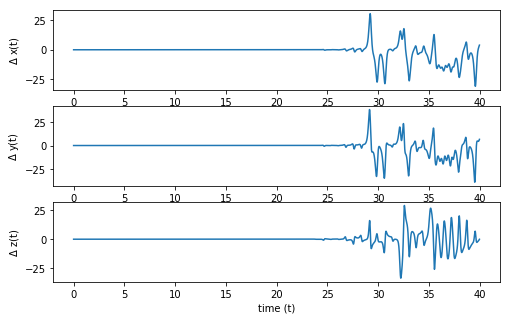
\includegraphics[scale=0.8]{Figures/delta_trajectory.png}
	\caption[An Electron]{The deviation of paths with start out very close to each other at tie $t=0$.}
	\label{fig:delta_trajectory}
\end{figure}
Fig. [\ref{fig:3d_trajectory}] shows a beautiful 3-D plot of the numerically integrated solution, which looks like the wings of a butterfly. Probably because of this, chaos is also sometimes referred to as the \textit{butterfly effect}.

Lorenz's model is so powerful that it continues to be studied till today. We shall investigate this further in the thesis, and hope to make some more comments in the final report.
\begin{figure}[h!]
	\centering
	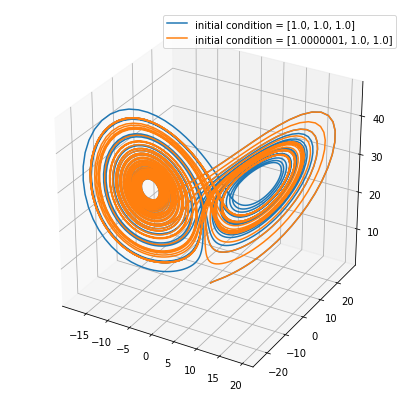
\includegraphics[scale=0.7]{Figures/3d_trajectory.png}
	\caption[An Electron]{A 3-D plot of $x,y,z$. Chaos is evident here too.}
	\label{fig:3d_trajectory}
\end{figure}
